\chapter{Tables}
\label{sec:tabelappendix}
 \section{Set-Up of Perturbation}
\begin{longtable}[H]{|l|c|c|c|}
    \hline 
    \multicolumn{4}{|l|}{\textbf{Perturbation settings}}\\
    \hline 
    \textbf{Variable} & \textbf{spatial correlation [km]} & \textbf{distribution} & \textbf{scaling factor} \\ 
    \hline
    $c_{ice}$ & 60000 & lognormal & 0.25 \\
    \hline
    $c_{snow}$ & 60000 & lognormal & 0.25 \\
    \hline
    $c_{rain}$ & 60000 & lognormal & 0.25 \\
    \hline
    $c_{lcw}$ & 60000 & lognormal & 0.25 \\
    \hline

    $c_{\mathrm{om}}$ &200000  & lognormal& Table \ref{tab:scale_aerosol} \\
    \hline
    $c_{\mathrm{bc}}$ & 200000  &lognormal & Table \ref{tab:scale_aerosol} \\
    \hline
    $c_{\mathrm{ss}}$ & 200000  & lognormal & Table \ref{tab:scale_aerosol} \\
    \hline
    $c_{\mathrm{sul}}$ & 200000  & lognormal & Table \ref{tab:scale_aerosol} \\
    \hline
    $c_{\mathrm{dd}}$ & 200000 &  lognormal &Table \ref{tab:scale_aerosol}  \\
    \hline
    $q_{\mathrm{spec}}$ & 60000  & normal & 2.00 \\
    \hline
    $\alpha_{\mathrm{om}}$ &60000  & normal&  1.00\\
    \hline
    $\alpha_{\mathrm{bc}}$ & 60000  &normal & 1.00 \\
    \hline
    $\alpha_{\mathrm{ss}}$ & 60000  & normal &  1.00\\
    \hline
    $\alpha_{\mathrm{sul}}$ & 60000  & normal & 1.00 \\
    \hline
    $\alpha_{\mathrm{dd}}$ & 60000  & normal & 1.00 \\
    \hline
    $\sigma_{\mathrm{om}}$ &60000  & normal& 0.1\\
    \hline
    $\sigma_{\mathrm{bc}}$ & 60000  &normal & 0.1\\
    \hline
    $\sigma_{\mathrm{ss}}$ & 60000  & normal &  0.1\\
    \hline
    $\sigma_{\mathrm{sul}}$ & 60000  & normal & 0.1\\
    \hline
    $\sigma_{\mathrm{dd}}$ & 60000  & normal & 0.1 \\
    \hline
    $c_{\mathrm{0,rain}}$ & 60000  & normal & 0.20 \\
    \hline
     $c_{\mathrm{0,lcw}}$ & 60000  & normal & 0.20 \\
    \hline
     $c_{\mathrm{0,ice}}$ & 60000  & normal & 0.20 \\
    \hline
     $c_{\mathrm{0,snow}}$ & 60000  & normal & 0.20 \\
    \hline
    $c_{\mathrm{1,rain}}$ & 60000  & normal & 0.20 \\
    \hline
     $c_{\mathrm{1,lcw}}$ & 60000  & normal & 0.20 \\
    \hline
     $c_{\mathrm{1,ice}}$ & 60000  & normal & 0.20 \\
    \hline
     $c_{\mathrm{1,snow}}$ & 60000  & normal & 0.20 \\
    \hline
     

    \caption{Namelist settings defining the patterns, constructed by the pattern generator, of the perturbed quantities. The spatial correlation provided, is only a namelist setting and has a complex relation to the actual spatial scale as described in Section \ref{sec:pattern gen}. It cannot be directly related with a length scale, because it is scaled with respect to the Earth's radius, since it as originally set-up for a global model. \label{tab:namelist_pert}}
\end{longtable}

\begin{landscape}
    \begin{longtable}{|l|c|c|c|c|c|c|c|c|c|c|c|c|}
            \hline 
            \multicolumn{13}{|c|}{  \textbf{Scaling Factors of Aerosol Perturbation} }\\
            \hline 
                   
              \textbf{Month}&\textbf{1}&\textbf{2}&\textbf{3}&\textbf{4}&\textbf{5}&\textbf{6}&\textbf{7}&\textbf{8}&\textbf{9}&\textbf{10}&\textbf{11}&\textbf{12}\\
            \hline 
            \hline
            Sulphate&1.3357& 1.5475 & 2.1818 & 2.8114 & 2.7717 &  3.1702 & 3.6221 & 3.4091 & 3.6193 & 3.0257 & 3.9347 & 4.4281 \\
            \hline
            Organic Matter & 4.3013 & 4.2449 & 4.0527 & 3.6794 &  4.3204 &  4.4870 & 3.7650 & 3.3974 & 3.0685 & 3.3869 & 3.5936 & 4.0124\\
            \hline
            Sea Salt&3.6922 & 3.3340 & 2.2834 & 2.0473 & 1.5699 &  1.4266 &  1.8392 & 1.7394 & 2.3499 & 2.7272 & 3.5206 & 3.1504 \\
            \hline
            Desert Dust& 3.4771 & 2.2858 & 2.5117 & 3.4750 &  4.1395 & 4.0536 & 3.5781 & 3.6066 & 3.9279 & 3.1142 &  2.4776 & 2.4406\\
            \hline
            Black Carbon &  5.2838&  5.3458 & 5.0817 & 4.7262 & 5.4137 & 5.6549 & 4.7267 & 4.2958 & 3.9782 & 4.2889 & 4.5131 & 4.9752 \\
            \hline
    \caption{Scaling factors  \label{tab:scale_aerosol} of the different aerosols. Set with respect to their global maxima}
    \end{longtable}
\end{landscape}

\section{Variables and Abbreviations}

\begin{longtable}[H]{|l|c|c|}
\hline 
\multicolumn{3}{|l|}{\textbf{Used Variables}}\\
\hline 
\textbf{Variable} &\textbf{Name} & \textbf{Unit} \\ 


\hline
$A$ & non-parametrized tendency & varies\\
\hline
$a_{0,i}$, $a_{1,i}$ & surface volume coefficients & $ \left[ \mathrm{ m^{2} \ kg^{-1}} \right]$, [none] \\
    \hline
$a^{s}_{n}$, $b^{s}_{n}$ & Mie coefficients& [none]\\
\hline
$B_{a}$ &brightness of the object& $ \left[ \mathrm{cd \ m^{-2}} \right] $\\
\hline
$B_{b}$ &brightness of the background & $ \left[ \mathrm{cd\  m^{-2}} \right] $\\
\hline
$B_{s}$ &brightness of scattered light & $ \left[ \mathrm{cd\  m^{-2}} \right] $\\
\hline
$c_{\mathrm{bc}}$ &mass concentration of black carbon & $ \left[ \mathrm{\mu g \ kg^{-1}} \right] $\\
\hline 
$C_{ext}$ &extinction cross section & $ \left[ \mathrm{m^{2}} \right] $\\
\hline
$c_{j}$ &constant parameters & varies\\
\hline 
$c_{\mathrm{ice}}$ &mass concentration of ice & $\left[\mathrm{ kg \ kg^{-1} }\right]$\\
\hline
$c_{\mathrm{lcw}}$ &mass concentration of liquid cloud water&$\left[\mathrm{ kg \ kg^{-1} }\right]$\\
\hline
$C$ & Contrast &[none]\\
\hline
$C_{p}$ &specific heat of air for constant pressure&[$\mathrm{ kg\ m^{2}\ 
K^{-1} s^{-2} }$]\\
\hline
$c_{\mathrm{snow}}$ &mass concentration of snow & $\left[\mathrm{ kg \ kg^{-1} }\right]$\\
\hline
$c_{\mathrm{rain}}$ &mass concentration of rain &$\left[\mathrm{ kg \ kg^{-1} }\right]$\\
\hline
$c_{\mathrm{om}}$ &mass concentration of organic matter & $ \left[ \mathrm{\mu g \ kg^{-1}} \right] $\\
\hline
$c_{\mathrm{ss}}$ &mass concentration of sea salt &  $ \left[ \mathrm{\mu g \ kg^{-1}} \right] $\\
\hline
$c_{\mathrm{sul}}$ &mass concentration of sulphates &  $ \left[ \mathrm{\mu g \ kg^{-1}} \right] $\\
\hline
$c_{\mathrm{dd}}$ &mass concentration of desert dust &  $ \left[ \mathrm{\mu g \ kg^{-1}} \right] $\\
\hline
$E$ & electric field vector &  [$\mathrm{V \ m^{-1}}$] \\
\hline
$\vec{e}_{r}$ &radial unit vector &  $ [ \mathrm{none}] $\\
\hline
${e}_{j}$ & prognostic model variabels &  varies\\
\hline
$\vec{F}$&dissipative forcing&[$\mathrm{kg \ m^{-1} s^{-2}}$]\\
\hline
$g$&gravitational constant&[$\mathrm{kg \ m^{-1} s^{-2}}$]\\
\hline
G&geometric factor& $ \left[ \mathrm{m^{2}} \right] $\\
\hline

$L_{\Psi}$& spatial correlation length&[km]\\
\hline
$m$ &zonal wave number& [none]\\
\hline
$M$ &source/sink term for humidity& $\left[\mathrm{ kg \ kg^{-1} \ s^{-1} }\right]$\\
\hline
$n$ &total wave number& [none]\\
\hline
$T$ &temperature& [$^{\circ}$ K]\\
\hline
$T_{x}$ &tendency of  x & varies\\
\hline
$p$ & pressure & [Pa] \\
\hline
$P$ &parametrized tendency & varies\\
\hline
$P_{x}$ &perturbation of  x & varies\\
\hline
$Q$ &heat& [J]\\
\hline
$ Q_{ext}$&extinction coefficient& [none]\\
\hline
$q_{\mathrm{rel}}$ &relative humidity& [none]\\
\hline
$q_{\mathrm{spec}}$ &specific humidity&$\left[\mathrm{ kg \ kg^{-1} }\right]$\\
\hline
$r$ &particle radius& [m]\\
\hline
$\vec{r}$ & radial vector& $ [m]$\\
\hline
$r_{j}$ &random number& [none]\\
\hline
$R$ &gas constant& $ \left[\mathrm{ kg \ m^{2}s^{-2} \ K^{-1} \ mol^{-1}} \right]$\\
\hline
$R_{\mathrm{E}}$ &average radius of the Earth& [km]\\
\hline
RPS &Ranked Probability Score & [none] \\
\hline
RPSS &Ranked Probability Skill Score & [none] \\
\hline
$s$ &scaling factor & [none] \\
\hline
SS &Skill Score & [none] \\
\hline
$t$ &time & [sec] \\
\hline
$\vec{v}$ & wind velocity& $\left[\mathrm{ m \ s^{-1} }\right]$\\
\hline
$\vec{V}$ & horizontal wind vector& $\left[\mathrm{ m \ s^{-1} }\right]$\\
\hline
$vv_{\mathrm{score}}$ &model score &[km]\\
\hline
$vis_{\mathrm{o}_{n}}$ & observed visibility value& [km]\\
\hline
$vis_{\mathrm{f}_{n}}$ &forecast visibility value &[km]\\
\hline
$z$ & height &[m]\\
\hline
$w$ & vertical wind component& $\left[\mathrm{ m \ s^{-1} }\right]$\\
\hline
$\alpha$ & scattering size parameter &[none]\\
\hline
$\alpha_{j}$ & attenuation coefficient of aerosols&$\left[\mathrm{ m^{2} \ g^{-1} }\right]$\\
\hline
$\beta_{\mathrm{a},j}$ & atmospheric extinction coefficient &[$\mathrm{km^{-1}}$]\\
     & of different aerosols &     \\
\hline
$\beta_{h,i}$ & atmospheric extinction coefficient  &[$\mathrm{km^{-1}}$]\\
& of different hydrometeors &\\
\hline
$\beta_{R}$ & atmospheric extinction coefficient  &[$\mathrm{km^{-1}}$]\\
& by Rayleigh scattering &\\
\hline
$\beta_{\mathrm{tot}}$ & atmospheric extinction coefficient&[$\mathrm{m^{-1}}$]\\
\hline
$\varepsilon$ &liminal contrast&[none]\\
\hline
$\kappa$ & Poisson constant & $\left[\mathrm{ mol^{-1} }\right]$\\
\hline
$\rho$ &density of air& $\left[\mathrm{ kg\ m^{-3} }\right]$\\
\hline
$\rho_{dry}$ &density of dry air& $\left[\mathrm{ kg\ m^{-3} }\right]$\\
\hline
$\sigma_{j}$ & scattering cross section of aerosols&$\left[\mathrm{ m^{2} }\right]$\\
\hline
$\lambda$ & wavelength & [m]\\
\hline
$\vec{\lambda}$ & Lyapunov vector& [$s^{-1}$]\\
\hline
$\lambda_{j}$ & Lyapunov exponent& [$s^{-1}$]\\
\hline
$\lambda_{\mathrm{lon}}$ & longitude & [$^{\circ}$]\\
\hline
$\phi$ & latitude &[$^{\circ}$]\\
\hline
$\Phi$ & geopotential &$\left[\mathrm{ m ^{2}\ s^{-2} }\right]$\\
\hline
$\Phi_{\mathrm{t}}$ & time dependent phase factor &[none]\\
\hline
$\vec{\Omega}$ & angular velocity & [none]\\
\hline
$\vec{\omega}$ & vorticity & [$s^{-1}$]\\
\hline

\caption{List of used variables \label{tab: variables}}
\end{longtable}

\begin{table}[h]
    \footnotesize
    \centering
        \begin{tabular}{|l|c|}
        \hline
        \textbf{Abbreviation and Symbols}&\textbf{Meaning}\\
        \hline
        \hline
        AROME&Application of Research to Operations on Mesoscale\\
        \hline
        ALADIN& Aire Limitée Adaptation Dynamique Développement International\\
        \hline
        ECMWF& European Centre for Medium-Range Weather Forecasts\\
        \hline
        EDA & Ensemble Data Assimilation\\
        \hline
        FFT & Fast Fourier Transformation\\
        \hline
        IFS&Integrated Forecast System \\
        \hline
        LAM&Limited Area Model \\
        \hline
        NWP & Numerical Weather Prediction\\
        \hline
        UTC & Universal Time, Coordinated\\
        \hline
        RMSE& Root Mean Squared Error\\
        \hline
        RMSLog & Root Mean Squared Difference of the Logarithmic values\\
        \hline
        RPS & Ranked Probability Score\\
        \hline
        RPSS & Ranked Probability Skill Score\\
        \hline
        WMO& World Meteorological Organization\\
        \hline
        WRF& Weather Research and Forecasting\\
        \hline
        $\Im$ & Imaginary part of a complex number\\
        \hline
        $\Re$ & Real part of a complex number\\
        \hline
        
    
    \end{tabular}
    \caption{List of abbreviations and symbols in this thesis}
    \label{tab:abbrivitations}
\end{table}

\begin{table}[h]
    \footnotesize
    \centering
        \begin{tabular}{|l|c|}
        \hline
        \textbf{SYNOP key}&\textbf{visibility [km]}\\
        \hline
0	& 0.00\\
\hline
1&	0.10\\
\hline
2 &  0.20\\
\hline
...& ..\\
\hline
49 & 4.90\\
\hline
50&	5.00\\
\hline
51&	none\\
\hline
...& ..\\
\hline
55& none\\
\hline
56&	6.00\\
\hline
57&	7.00\\
\hline
...& ..\\
\hline
79&	29.00\\
\hline
80&	30.00\\
\hline
81&	35.00\\
\hline
...& ..\\
\hline
88&	70.00\\
\hline
89&	more than 70\\
\hline

    \end{tabular}
    \caption{SYNOP keys: Numeric system used by the human observers to encode visibility}
    \label{tab:synoptable}
\end{table}

\chapter{Images}
\label{sec:imagesappendix}
\section{Surface Weather Analysis}
\begin{figure}[H]
    \centering
    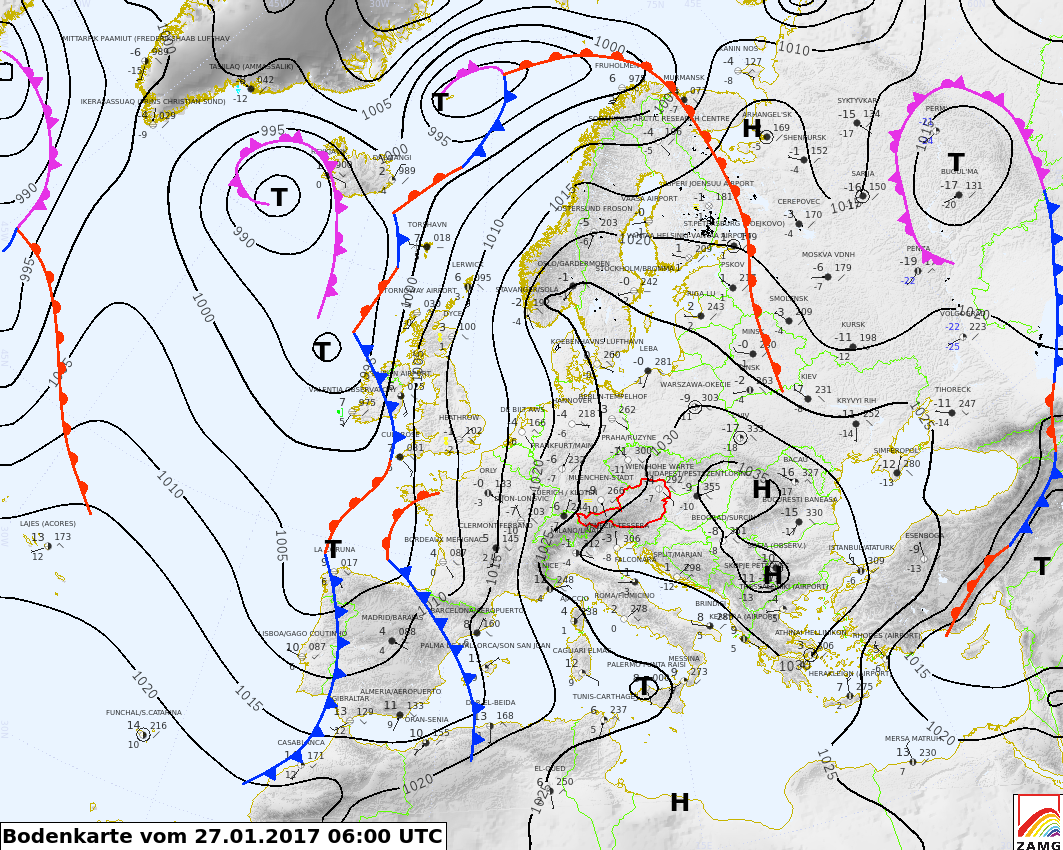
\includegraphics[width=\textwidth]{graphics/Bodenkarte0600.png}
    \caption[Surface Weather Analysis 06:00 UTC]{Surface weather analysis 27-01-2017, 06:00 UTC of Europe. Image from the online archive of `\citeauthor{zamg}'  \cite{zamg}.}
    \label{fig: Bodenkarte06}
\end{figure}

\begin{figure}[H]
    \centering
    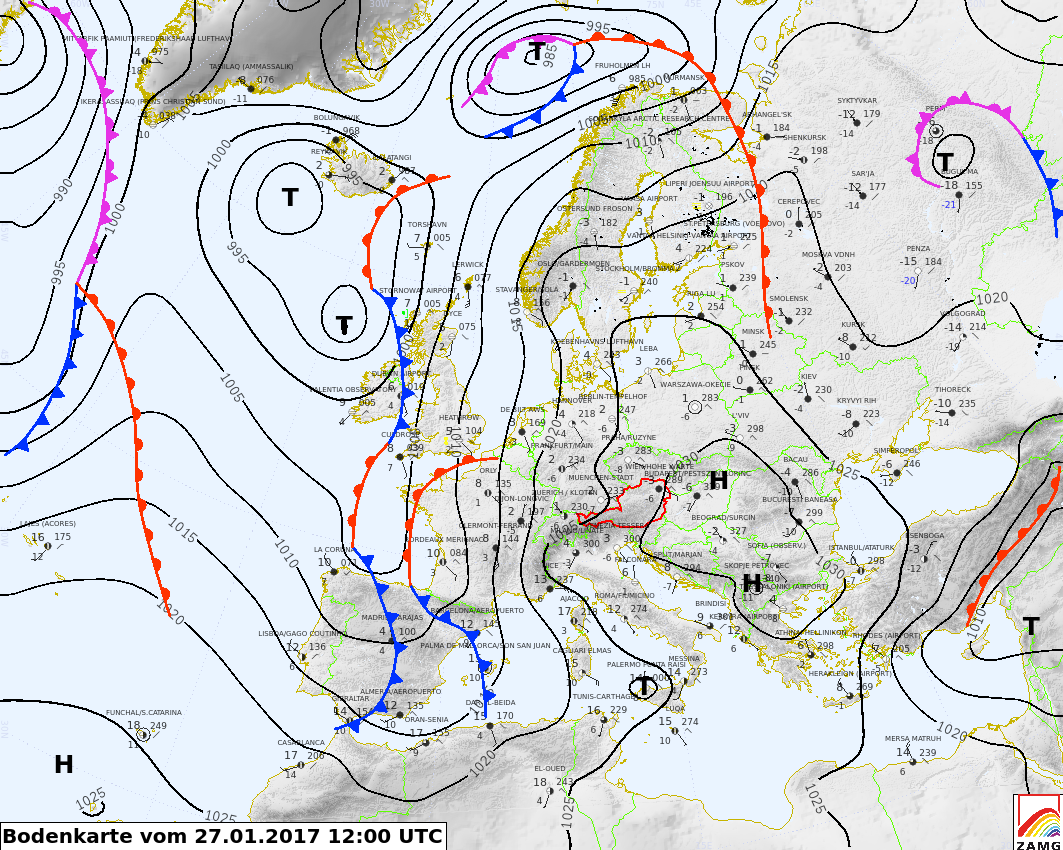
\includegraphics[width=\textwidth]{graphics/Bodenkarte1200.png}
    \caption[Surface Weather Analysis 12:00 UTC]{Surface weather analysis 27-01-2017, 12:00 UTC of Europe. Image from the online archive of `\citeauthor{zamg}'  \cite{zamg}.}
    \label{fig: Bodenkarte12}
\end{figure}